\documentclass[a4paper,twocolumn]{article}
\usepackage{listings}
\usepackage{amsmath}
\usepackage{tikz}
\usepackage{sectsty}
\bibliographystyle{plain}

\title{Dominance is not a Tree \\
\Large{Towards More Precise Dominance Relations}}
\date{Jan 25, 2024}
\author{George Stelle \; Tarun Prabhu \; Pat McCormick \\ Los Alamos National Laboratory}

\lstdefinestyle{mystyle}{
  basicstyle=\ttfamily
}
\lstset{style=mystyle}
\sectionfont{\fontsize{12}{15}\selectfont}

\begin{document}
\maketitle

In LLVM and other modern compilers, single static assignment (SSA) is a crucial
theory for internal representations, enabling optimizations in the presence of
imperative code. A fundamental function of SSA is calculating and using
dominance relations to determine where immutable variables can be referenced.
Dominator trees have historically been a good approximation of the dominator
relation and efficiently computable. However, there are programs for which the
dominator tree fails to capture precise dominance relations, preventing
optimizations. In this work, we will give examples of these kinds of programs,
and show how removing the restriction to tree relations enables more precise
dominance relations, therefore enabling more optimization. We discuss how one
can use properties of SSA to implement a more general dominance relation using
a small set of trees corresponding to shared branches, which we call a
dominator \emph{grove}. We present a work-in-progress implementation of a
dominator grove in LLVM, along with some of the current hurdles in modifying
the existing analyses and transformations to be sound in the presence of
non-tree dominance relations. Using the implementation, we collect empirical
data on the frequency of non-tree dominance relations in real code. We present
some basic formal properties of the approach, and end with a discussion of
future work, including concurrent extensions to SSA theory.  

\section*{Motivation}
Recall the definition of dominance in the context of programs: a node $a$
dominates a node $b$ if every \emph{valid} path from the entry block to $b$ goes
through $a$. Note that we specify valid paths explicitly, as historically
dominance has focused on any path through the control flow graph (CFG).
Because we care about dominance in \emph{programs}, we need to reason about
valid paths beyond just the CFG. 

To understand non-tree dominance relations, consider the following example: 
\begin{minipage}{\linewidth}
\begin{lstlisting}[language=C]
void f(bool c, int x){
  int y = 0;         \\ entry
  if(c) y = pre(x);  \\ pre
  body(x);           \\ body	
  if(c) post(y);     \\ post
}
\end{lstlisting}
\end{minipage}
Note that there are two valid paths through the function: one which calls
\texttt{pre} and \texttt{post} and one which doesn't. Therefore, by the
definition of dominance, the call to \texttt{post} is dominated by the call to
\texttt{pre}. Representing the dominance relations graphically gives: 
\begin{center}
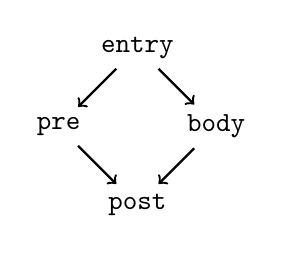
\begin{tikzpicture}[->, line width=0.3mm]
\node(entry) at (2,3) {\texttt{entry}};
\node(a) at (1,2) {\texttt{pre}};
\node(b) at (3,2) {\texttt{body}};
\node(c) at (2,1) {\texttt{post}};
\path
(entry) edge (a)
(entry) edge (b)
(a) edge (c)
(b) edge (c);
\end{tikzpicture}
\end{center} 
which is clearly not a tree. When a dominator tree is used, because of the
failure to capture that \texttt{pre} dominates \texttt{post}, the value of
\texttt{y} cannot be referenced in \texttt{post}, leading to potentially
missed opportunities for optimization.

\section*{Implementation}
The crucial property that lets us refine the notion of valid paths and
therefore refine the dominance relation is that whenever there are multiple
conditional branches that share a immutable condition variable $c$, we can construct
two distinct dominator trees for cases where $c=0$ and $c=1$. If a dominance
relation holds for both dominator trees, then it holds in the general case. We
call this structure a dominator \emph{grove}, as it contains a small set of
trees. Because of this dependence on condition variables, one can view this
approach as a class of \emph{context-sensitive} dominance relations. This is in
contrast to the dominator tree, which is computed from the CFG, and no further
context.

We present an initial implementation of the dominator grove approach in LLVM.
By modifying the existing implementation of incremental dominator tree updates,
we show how one can extend the implementation of dominator trees to implement
dominator groves in a way that requires only a relatively small change to the
codebase.\cite{georgiadis2012experimental}

While the implementation successfully computes more precise dominance
relations, there is a problem: the extra precision appears to break existing
analysis and transformation passes. While we're still not sure what causes all
of the issues, we believe it to be due to assumptions about the structure of
dominance. These assumptions are violated by the more precise dominance
relations, causing compiler bugs. We hope to discuss some of the challenges in
removing these assumptions from LLVM, and to get feedback from the community on
the cost of addressing these assumptions.

\section*{Empirical Measures}
In the above example we've shown the existence of programs with non-tree
dominance relations, but a natural question is how often these kinds of
programs occur in the wild. To measure this, we run the implementation
described above on \texttt{llvm-test-suite}. We discover that out of the
$\approx55$ million calls to \texttt{dominates}, $\approx1.9$ million calls are made
more precise by the dominator grove, or $\approx3.5\%$. This shows that there are
a non-trivial number of non-tree dominance relations in real world code. We
look forward to discussing a further breakdown of the data with the community.

\section*{Verification}
In the interest of ensuring correctness of the approach, we've proved a number
of simple but important properties. First, and most obviously, every valid path 
through the program is a valid path through the CFG. Next, following direcly
from the above property, every dominator grove relation is at least as precise 
as a dominator tree. In other words, if a relation holds for the dominator tree, 
then it holds for the dominator grove. This ensures that we are never
decreasing the amount of dominance relations that can be used to enable
optimizations.

\section*{Concurrency}
In addition to improving optimizations for sequential programs, we argue that 
removing the tree constraints from dominance relations is necessary to build a
concurrent SSA theory. To be able to run two pieces of code concurrently, then
wait for them to finish, we need to be able to represent that neither dominate
each other, but both dominate the join point. We look forward to discussing
with the community further how SSA and LLVM can be extended with concurrent
semantics.

\section*{Future Work}
While adding the ability to compute more precise dominance relations requires
a fairly small change, it's not clear how much existing code that assumes a 
dominator tree structure in analysis and transformation passes will need to be
changed. We hope to get feedback from the community on how best to move forward
to maximize likelihood of getting the approach integrated into LLVM. 

\bibliography{refs}

\end{document}
